
%% ==============
\chapter{Photon-based Next Event Estimation}
\label{ch:PNEE}
%% ==============

We propose a novel approach to find estimators for importance sampling (especially) for scenes with many localized light sources. Our key goal is to efficiently reduce the variance $\sigma$ (section~\ref{sec:IS}) \unsure{ref to sections?} of the direct lighting term of our Monte Carlo integrator (section~\ref{sec:MC}) by estimating the strength of the light contribution from every light source. Typically ruling out light sources that contribute nothing (zero contribution paths) due to shadowing has a significant impact.

In a preprocess all light sources scatter out photons into the scene, similar to photon mapping \cite{jensen2001realistic}, but no bounces are considered, as we only need direct light paths for our Next Event Estimation estimator. Further, we only consider LD paths, all LS*D paths are disregarded. Those paths are disregarded by the first condition anyway, but we want to emphasize that refractions of any kind make a photon obsolete for our usecase. After the photons are scattered out into the scene we are looking for efficient ways to approximate or store those photons. Contrary to techniques like proposed by \cite{Estevez} where we build up our datastructures around the light sources themselves, with PNEE we build the datastructures around the light-receiving parts of our scene. This generally will scale up the data that needs to be processed but at the same time bear opportunity to refine our estimators. Then, the last step happens from within our pathtracer, we produce an estimator for our Next Event Estimation at every intersection by accessing and processing surrounding photons or CDFs.

Note that when the photon count goes towards infinity and the intersection search radius goes towards zero the estimator becomes the direct lighting term we are trying to find, making the Monte Carlo integration obsolete. As we are bound by time and memory, the key challenge is to find a good approximation thereof in minimal time. We found that shooting, processing and storing photons in the preprocess is not as tightly bound, but the lookup thereof in the integrator is very timecritical as it runs once for each intersection in the pathtracer. In the following sections we discuss various datastructures and storing methods we explored throughout this work.



\section{Mix and match}

Throughout this work we explored several techniques that trade off time, memory and image quality (visible artifacts)\footnote{As all our techniques are unbiased, images always converge against the same result. In practice those artifacts converge almost never, thus we list artifacts, even though they just can be seen as an unproportional time tradeoff.}. From a meta-perspective we can divide our technique into several subprocesses:

\begin{itemize}
    \item shoot photons (section~\ref{ch:shootph})
    \item store those photons in some form (section~\ref{ch:formofstorage})
    \item add this information into a fitting acceleration datastructure (section~\ref{ch:AccelDat})
    \item and finally, from within the path tracer, retrieve this information and potentially interpolate it to construct meaningful estimators (section \ref{ch:interpolation})
\end{itemize}

For each subprocess we present several ideas, where mostly any permutation of those ideas could be utilized. Unsurprisingly, there are several natural fits, which we describe in more detail, have implemented and evaluate against each other and known techniques in section~\ref{ch:Evaluation}. We refer to the implemented techniques as \textit{cdfgrid}, \textit{photontree} and \textit{cdftree}. All of which have specific peculiarities and parameters which are introduced during the course of this work. Table \ref{tb:techniques} gives an overview of subtechniques and colors indicate which of those are implemented with the respective technique. We advise the reader to refer back to this overview, to put newly introduced techniques into perspective.
\unsure{good table and styling?}

\begin{center}


\newcommand{\tdot}[1]{ \tikz\draw[#1,fill=#1] (0,0) circle (.5ex); }
\ra{1.3}
\begin{tabular*}{\textwidth}{@{}l @{\extracolsep{\fill}} lll@{}}\toprule
shooting photons & form of storage & datastructure & interpolation \\ \midrule

uniform \tdot{yellow}\tdot{blue}\tdot{green}        & photons \tdot{blue}               & hashed grid \tdot{yellow}                 & none \tdot{yellow}\tdot{blue}\tdot{green}\\
powerbased \tdot{yellow}\tdot{blue}\tdot{green}     & lightcuts                         & k-d tree \tdot{blue}\tdot{green}          & trilinear \tdot{yellow} \\
importance sampling                                    & CDFs \tdot{yellow}\tdot{green}    & Octree                                 & shepard \tdot{blue}\tdot{green}\\
                                                    &                                   &                                           & K. Regression\footnote{Stricktly speaking Kernel Regression is an approximation rather than an interpolation.} \tdot{blue}\tdot{green} \\
\bottomrule
\multicolumn{4}{c}{cdfgrid \tdot{yellow} \qquad photontree \tdot{blue} \qquad cdftree \tdot{green}} 
\end{tabular*}
%\captionof{table}{Various subtechniques introduced throughout this work. Colors indicate which subtechnique was implemented with the respective technique. }
\label{tb:techniques}
\end{center}




\section{Shooting photons}
\label{ch:shootph}
The first step in the preprocess is to scatter out photons. We rely on the same theoretical basis as photon mapping (section \ref{sec:PM}) but without producing any kind of bias as long as our CDFs always inherit every light source. We generate photons at the scenes light sources and intersect them with our scene geometry. We sample the light source $x$ and a point s and direction $\omega$ on that light source with respect to a probability distribution. This bears opportunity to guide the generation of photons to maximize the photon density in the important parts of the scene. Let $L(s,\omega)$ be the radiance \unsure{radiance?} at point s in direction $\omega$, $p(x)$ the probability to sample light source $x$ and $p(\text{s}, \omega)$ the probability to sample the ray, the flux $\beta$ of this photon is calculated as follows.

\begin{align}\label{eq:beta}
\beta = \frac{|\cos{\omega}|L(\text{s}, \omega)}{p(x)p(\text{s}, \omega)}
\end{align}

The basic approach is to use uniform CDFs to sample both $p(x)$ and $p(\text{s}, \omega)$. We found that results can be greatly enhanced for typical (but not all) scenes by sampling $x$ based on the light power. We elaborate differences in section \ref{ch:}\todo{input section}. In the future it might be of value to migrate sampling strategies presented for photon mapping to PNEE, see \cite{DBLP:conf/rt/SuykensW00}\todo{add more}. After we found the first intersection of the photon we check the surface BSDF, if it is fully specular, the photon can be discarded, if it has a diffuse part we store the photon, or at least its origin and $\beta$ in a data structure which we discuss in the next sections.

\section{Form of storage}
\label{ch:formofstorage}

\subsection{Photons}

Storing every photon with its weight and potentially additional data like the direction it came from is the most precise form to later compute our estimator, as the number of datapoints corresponds to our photon count. For every intersection point we evaluate the surrounding photons and compute an individual cumulative distribution function. As the photon count is quite high, typically several million unevenly distributed datapoints, the lookup is a bottleneck in this case, even with acceleration structures like a k-d tree that we discuss in section~\ref{sec:pneekdtree}. Nonetheless, the approach is worthwhile due to the potential quality of the estimator.

If we want to lessen the strain on the integrator, we might reduce the number of datapoints within the preprocess and store an approximation instead of every individual photon. We accumulate the $\beta$ per light sample $x$ within a defined area. Then this map of weights is transformed into a lightcut or CDF.

\subsection{Lightcut}

Recent work from Estevez and Kulla \cite{Estevez} and Vévoda and Křivánek \cite{Vevoda} rely on lightcuts. A lightcut is a horizontal cut through a lighttree (essentially a binary tree with light sources as leafs) and has the advantage of being very compact when many adjacent leafs of the subtree have the same sampling probability. This is quite typical, as most of the times only a small portion of lights contribute to a given point, while all other lights are shadowed. Let $n$ be the number of lights and $c$ the size of the cut. $c$ can be anything between one, cutting once at the root node, and $n$, cutting each leaf. Lightcuts thus adapt to the complexity of the given datapoint and often can be stored quite compact. Sampling from such a cut runs in $\bigO(\log{n})$ but on avarage in $\bigO(\log{c})$, size of the lighttree is $\bigO(n\log{n})$. The advantages of lightcuts break down when there are none or few adjacent samples that share the same probability. Proposed algorithms by Estevez \cite{Estevez} and others to find such a cut, in our view, have similarities to unsupervised machine learning algorithms, where the lighttree is a dendrogram of a cluster (typically produced by agglomerative hierarchical clustering) and the algorithm tries to assign a label (the probability) to the lights based on their cluster affinity. 

\subsection{CDF}

Another possibility is to directly store cumulative distribution functions during the preprocess. A CDF is usually stored as an sorted array of float values that grow from 0 to 1, the size is fixed at $n$, and sampling is done in $\bigO(\log{n})$. With our technique we found lightcuts not well fitting, as rather than making broad approximate statements about clusters of lights, we dominantly have individually distinct contributions accumulated through photons. Let $k$ be the number of contributing light sources to a particular CDF, which equals to all light sources with a sampling probability unequal to zero. This would degenerate a lightcut into a CDF where $c \approx k$. Especially when creating CDFs within the integrator a linear space and timecomplexity is generally unacceptable. We observe that most of the time $k$ is significantly smaller than $n$ due to localized light influences. To address this issue we present Sparse CDFs in section~\ref{sec:sparse} where space- and time complexity for construction is $\bigO(k)$ and sampling is $\bigO(\log{k})$. Furthermore, in section \ref{sec:intcdf} we introduce the possibility to sublinearly interpolate between any kind of CDFs in $\bigO(d)$ space and time for construction and $\bigO(d + \log{n})$ sampling, where $d$ is the number of interpolated CDFs.
%TODO: Wie tief soll ich hier gehen wieso das so ist?

\subsubsection{Sparse CDF}
\label{sec:sparse}
\begin{figure}[htb] 
	\centering
    \begin{tikzpicture}[scale=7, cdf/.style ={thick}]

    
    %zoom lines
    \draw (0,0) -- (0,-0.2);
    \draw (1,0) -- (0.8,-0.2);
    

    %cdfs, lines and filling
    \draw[thick, fill=green!10] (0,0) rectangle (0.25, 0.1) node[pos=.5] {25\%};
    \draw[thick, fill=red!10] (0.25, 0) rectangle (0.5, 0.1) node[pos=.5] {25\%};
    \draw[thick, fill=blue!10] (0.5, 0) rectangle (1, 0.1) node[pos=.5] {50\%};
    
    \draw[thick, fill=green!10] (0, -0.3) rectangle (0.2, -0.2) node[pos=.5] {20\%};
    \draw[thick, fill=red!10] (0.2, -0.3) rectangle (0.4, -0.2) node[pos=.5] {20\%};
    \draw[thick, fill=blue!10] (0.4, -0.3) rectangle (0.8, -0.2) node[pos=.5] {40\%};
    
    \draw[thick, fill=black!10] (0.8, -0.3) rectangle (1, -0.2);
    
    \fill[fill=green!10] (0.84, -0.3) rectangle (0.86, -0.2);
    \fill[fill=red!10] (0.88, -0.3) rectangle (0.9, -0.2);
    \fill[fill=blue!20] (0.98, -0.3) rectangle (1, -0.2);
    
    \foreach\x in {0.82,0.84,...,0.98}
        \draw (\x,-0.2) -- (\x,-0.3);
        
    \draw[cdf] (0,0) rectangle node[left=4cm] {Inner CDF} (1,0.1);
    \draw[cdf] (0,-0.3) rectangle node[left=4cm] {Sparse CDF} (1,-0.2);
    
    % b range indicators
    \draw[thick] (0, -0.16) -- node[above] {$1-b = 0.8$} (0.8, -0.16) ;
    \draw[thick] (0, -0.17) -- (0, -0.15);
    
    \draw[thick] (0.8, -0.16) -- (1, -0.16) node[above] {$b = 0.2$} ;
    \draw[thick] (0.8, -0.17) -- (0.8, -0.15);
    \draw[thick] (1, -0.17) -- (1, -0.15);
    
    % braces
    \draw[line width=1.25pt, decoration={calligraphic brace,amplitude=7pt,mirror,raise=6pt},decorate]
                    (0,-0.3) -- node[below=12pt] {$k = 3$} (0.8,-0.3);
    \draw[line width=1.25pt, decoration={calligraphic brace,amplitude=7pt,mirror,raise=6pt},decorate]
                    (0.8,-0.3) -- node[below=12pt] {$n$} (1,-0.3);
    \draw[line width=1.25pt, decoration={calligraphic brace,amplitude=7pt,mirror,raise=26pt},decorate]
                    (0,-0.3) -- node[below=32pt] {$n$ distinct samples} (1,-0.3);

\end{tikzpicture}
    \caption{A sparse CDF either samples from the uniform part with probability $b$ or from the inner CDF with probability $1-b$. $k$ are the number of samples that have a non-zero probability in the non-uniform part. All $k$ samples are repeated within the uniform part to facilitate calculations of $p_{\text{sparse}}$ (equation \ref{eq:psparse}). The samples in sparse CDF are not in the correct order, as a result two additional hashmaps are needed.} 
    \label{fig:sparseCDF}
\end{figure}

We need \unsure{we need?} a CDF where only particular values from $0$ to $n$ may be sampled. We achieve this by using a classic CDF (inner CDF) with length $k$ and a hashmap which maps values $[1,k]\to [1,n]$\footnote{As the pre-image in $[1,k]\to [1,n]$ is a sequence this could also be a simple array instead of a hashmap. Before constructing the sparse CDF the photons are collected by some algorithm without knowing $k$ beforehand. As photons can originate from all $n$ light sources a hashmap is needed anyway. We continue with this hashmap to spare the conversion.}. After we sampled a number the map will map the sampled number to the original sample number. Further we also need a backmap which is the reverse of the former map. The backmap is used when you want to know the probability of a given original sample number $x$. The original sample number is mapped to the sample number that it corresponds to in the inner CDF, so the inner CDF can be queried for the corresponding probability. We additionally want to provide a base floor probability $b$, which is split equally by all $n$ light sources. Let $N$ be the set of all $n$ sample numbers and $K$ be the set of non-zero probability samples. The probability that a given sample $x$ is sampled by the sparse CDF is given as follows.
\begin{align}\label{eq:psparse}
 p_{\text{sparse}}(x) = 
\begin{dcases}
    p_{\text{inner}}(\text{backmap}(x))(1 - b) + \frac{b}{n},& \text{if } x \in K\\
    \frac{b}{n}, & \text{otherwise}
\end{dcases}
\end{align}
Even though we seemingly introduce unnecessary variance with this uniform base, it is absolutely crucial as we otherwise would introduce bias whenever our estimator would "forget" a light source, which is not uncommon for e.g. very distant or highly occluded light sources. Apart from that fact, it generally helps in areas where our estimator is bad for any reason, therefore the choice of $b$ should not be minimal, but rather roughly proportional to the expected quality of the estimator.

Construction is done in $\bigO(k)$ space and time, sampling in $\bigO(\log{k})$. Comparing to lightcuts we have a simpler datastructure in hand, that rules out non contributing light samples effectively. If we assume that equal non-zero probabilities are rare, which should be the case with many photon contributions, we generally should outperform lightcuts, especially because sampling the dominant case $x \notin K$ runs in $\bigO(1)$. 

\subsubsection{Interpolated CDF}
\label{sec:intcdf}
\begin{figure}[htb] 
	\centering
    \begin{tikzpicture}[scale=4.5, cdf/.style ={thick}]
    \small
    %zoom lines
    \draw (-1.1,0) -- (0,-0.4);
    \draw (-0.1,0) -- (0.4,-0.4);
    \draw (0,0) -- (0.4,-0.4);
    \draw (1,0) -- (0.9,-0.4);
    \draw (1.1,0) -- (0.9,-0.4);
    \draw (2.1,0) -- (1,-0.4);
    
    \draw[cdf] (-1.1,0) rectangle (-0.1,0.1);
    \draw[cdf] (0,0) rectangle (1,0.1);
    \draw[cdf] (1.1,0) rectangle (2.1,0.1);
    \draw[cdf] (0,-0.5) rectangle (0.4,-0.4);
    \draw[cdf] (0.4,-0.5) rectangle (0.9,-0.4);
    \draw[cdf] (0.9,-0.5) rectangle (1,-0.4);
    
    %cdfs, lines and filling
    \draw[thick, fill=green!10] (-1.1,0) rectangle (-0.6, 0.1) node[pos=.5] {50\%};
    \draw[thick, fill=red!10] (-0.6, 0) rectangle (-0.35, 0.1) node[pos=.5] {25\%};
    \draw[thick, fill=blue!10] (-0.35, 0) rectangle (-0.1, 0.1) node[pos=.5] {25\%};
    
    \draw[thick, fill=green!10] (0,0) rectangle (0.6, 0.1) node[pos=.5] {60\%};
    \draw[thick, fill=red!10] (0.6, 0) rectangle (0.9, 0.1) node[pos=.5] {30\%};
    \draw[thick, fill=blue!10] (0.9, 0) rectangle (1, 0.1);
    
    \draw[thick, fill=green!10] (1.1,0) rectangle (1.35, 0.1) node[pos=.5] {25\%};
    \draw[thick, fill=red!10] (1.35, 0) rectangle (1.4, 0.1);
    \draw[thick, fill=blue!10] (1.4, 0) rectangle (2.1, 0.1) node[pos=.5] {70\%};
    
    \draw[fill=green!10] (0,-0.5) rectangle (0.2,-0.4) node[pos=.5] {20\%};
    \draw[fill=red!10] (0.2,-0.5) rectangle (0.3,-0.4);
    \draw[fill=blue!10] (0.3,-0.5) rectangle (0.4,-0.4);

    \draw[fill=green!10] (0.4,-0.5) rectangle (0.7,-0.4) node[pos=.5] {30\%};
    \draw[fill=red!10] (0.7,-0.5) rectangle (0.85,-0.4);
    \draw[fill=blue!10] (0.85,-0.5) rectangle (0.9,-0.4);
    
    \draw[fill=green!10] (0.9,-0.5) rectangle (0.925,-0.4);
    \draw[fill=red!10] (0.925,-0.5) rectangle (0.93,-0.4);
    \draw[fill=blue!10] (0.93,-0.5) rectangle (1,-0.4);
    
    \draw[thick] (0.55,-0.39) node[above] {$\xi = 0.55$} rectangle (0.55,-0.41);
    
    \draw[thick] (0.3, 0.11) node[above] {$\xi = 0.3$} rectangle (0.3,0.09);
    
    \node at (0.5, -0.75) {$p_{\text{interpolated}}(1) = \overbracket{(0.5 * 0.4)} + \overbracket{(0.6 * 0.5)} + \overbracket{(0.25 * 0.1)} = 52.5\%$};
    
    \draw[->] (0.1,-0.5) -- (0.196,-0.65);
    \draw[->] (0.55,-0.5) -- (0.615,-0.65);
    \draw[->] (0.9125,-0.5) -- (1.05,-0.65);
    
    % pi range indicators
    \path (-0.2, -0.25) node[above] {$c_1 = 0.4$};
    \path (0.55, -0.25) node[above] {$c_2 = 0.5$};
    \path (1.25, -0.25) node[above] {$c_3 = 0.1$};
    
\end{tikzpicture}
    \caption{Three CDFs should be interpolated with corresponding weights $c_i$. Randomnumber $\xi$ is $0.55$. The second CDF is chosen, $\xi$ is cut and normalized to $0.3$. Sample 1 (green) is chosen. $p_{\text{interpolated}}$ is calculated according to equation \ref{eq:pinter}.} 
    \label{fig:interpolatedCDF}
\end{figure}

Suppose we want to sample a number from an interpolation between $d$ CDFs. A naive approach to achieve this is to loop through every CDF and for every sample add up the weights, normalize them in the end and store this as the new interpolated CDF. Construction would then run in $\bigO(d * n)$ and $\bigO(n)$ space, sampling in $\bigO(\log{n})$. As we will need the construction to run for every intersection in our scene it is unsustainable to have it run linearly in $n$. We propose a CDF interpolation scheme that constructs in $\bigO(d)$ time and space, with only minimal drawback when sampling with $\bigO(d + \log{n})$.

We receive a list of CDFs to interpolate and corresponding weights. We loop through the weights and normalize them, thus constructing an usual CDF that will sample $i \in [1,d]$. We keep an array of references to the base CDFs. Now, for the lookup we sample $i$ in $\bigO(\log{d})$ and then choose the $i'th$ CDF and sample within the CDF in $\bigO(\log{n})$. We now have the sample $x$ and also have to calculate the probability that $x$ was sampled. Let $c_i$ be the probability to sample the $i'th$ CDF and $p_i(x)$ the probability of sampling $x$ within the $i'th$ CDF, we calculate the probability as follows.

\begin{align}\label{eq:pinter}
    p_{\text{interpolated}}(x) = \sum_{i=1}^{d}p_{i}(x) \cdot c_i
\end{align}

The time complexity for this calculation is $\bigO(d)$, resulting in overall complexity $\bigO(\log{d} + \log{n} + d) = \bigO(d + \log{n})$. The whole process is illustrated in figure \ref{fig:interpolatedCDF}. Note that with our construction all base CDFs are required to have the same number of samples $n$ in the exact same order. This restriction might be lifted with additional maps, similar to sparse CDFs, but we have no need for it, as all our used CDFs have the same $n$ lights, thus we spare the overhead.

\section{Acceleration datastructure}
\label{ch:AccelDat}

After choosing what we store we are choosing how we store and access it from within our integrator. A critical part of finding our estimator is to access the data we previously stored. It is important to keep the probable distribution of photons in mind. Usually large parts of the scene won't have any photons and then there will be photon clusters, typically distributed on 3D-planes. Further, a typical problemcase for the choice of acceleration datastructures is called "teapot in a stadium" \todo{illustration?}. It describes the potentially vastly varying level of detail in a scene. The "teapot" is a small, highly detailed object in the "stadium" which is big, simple and mostly empty. This bears a typical trade off between adaptive datastructures like octrees or k-d trees, which handle varying LOD quite well, but generally have slower access times and static datastructures like a hashed grid, which has fast constant access times, but can't adapt to LOD at all. For our renderer often times not even the big $\bigO$ runtime is critical, but the constant overhead can be problematic, too. The best choice is often scene dependent, nonetheless, we are trying to find a good middleground that solves typical problem cases in photorealistic scenes. The form of storage does also impact the effectiveness of the acceleration datastructure, we present natural fits in the following chapters.

\subsection{Hashed grid}
\label{ch:pnee:hashedgrid}
Storing photons directly into a hashed grid is quite dangerous, almost any scene will have clusters of photons, sometimes consisting of a large portion of the total photon count. When doing a nearest neighbour lookup of our intersection point this can degenerate to linear run time complexity, not even in the light source count $n$, but in the total photon count. It is apparent that this is unacceptable, as even a small detail in the scene could blow up rendering times.

The idea here is to store exactly one CDF in the middle of each grid cell and using the clamped position as the key. Doing so, we utilize the constant access times of the hashed grid without the threat of photon clusters. At the same time we are giving up precision, as we loose all positional data of the photons. We do not interpolate the photons by distance to the CDF, rather every photon contributes at the same rate to this homogeneous grid cell. As every intersection point will clearly choose one CDF, this leads to sometimes very apparent variance cliffs at the edges of the grid cells (see figure \ref{fig:varianceEdge}). PBRTs \cite{pbrt} and Vevodas \cite{Vevoda} \unsure{use cite here or ref to the section where I introduced the technique?} technique have the exact same problem, but their CDFs transition somewhat smoothly as only position and angles are used for CDF calculation. The problem is highly accelerated with our technique because we inherit occlusion in the CDF generation which can create sharp edges in certain situations. We tackle this problem in section \ref{ch:trilinear}.


\subsection{k-d tree}
\label{sec:pneekdtree}

A k-d tree does fit much better when it comes to storing photons in a scene with potentially high variance in LOD. Construction of the tree is well studied, we thus throughout this work relied on Nanoflann \cite{blanco2014nanoflann}\unsure{implementation detail ok here?}, a highly optimized C++ k-d tree framework. After the photons are stored in the tree, the time critical part happens from within the integrator. 

A k-d tree can be queried for it's nearest neighbours or a defined radius. We tried both techniques, which vary mostly on how we interpolate the photons to construct the CDF. A NN-lookup has the advantage that in sparsely populated areas enough photons are always count to construct a somewhat meaningful CDF. Imagine a very distant object where only a few photons land, a radius-lookup might produce sharp variance edges where no photons are found, compared to regions where one or a few photons are found. With the radius-lookup the radius instead of the photon count is fixed, this helps fine tuning the interpolation kernels and allows unlimited number of lights to influence a point. Imagine a point where several thousands lights influence it's shading, a NN-lookup would construct a CDF with at maximum the number of lights of nearest neighbours, not even accounting for photons from the same light source. Finding an arbitrary amount of photons within a radius might get a problem performance wise, too. In extreme cases we suffer from similar problems like a hashed grid with a fixed radius with worse lookup times. Either the choice of radius or nearest neighbours becomes a critical parameter for the described scenarios. As photon density also depends on total photon count, both parameters are also influenced by the total photon count, which further complicates the issue. Considering the fact, that it is rare that so many light sources influence a point and even if so, individual contributions are low and likely somewhat uniform\footnote{Strong light sources will also dominate in the photon count. So if photons are uniform the result will likely be uniform. But there may be exceptions to this with sharp angles or very spiky BSDFs.}, thus this drawback will rarely cause problems. Not knowing the radius can be handled by the interpolation scheme, where for example modified shepard (section \ref{sec:modshep}) adapts to the maximum radius to smoothly phase the furthest photon in and out. From a theoretical standpoint we expect NN-lookups to be the more stable technique, still both have their pitfalls. Further analysis on this behaviour is made in section \ref{ch:ev:photontree}.

No matter which lookup method we choose we have to collect the accumulated $\beta$ per light. If we want to avoid running linearly in the number of lights, we have to use a hashmap mapping from light number to its $\beta$ in combination with the sparse CDF (\ref{sec:sparse}). Let the number of collected photons be $u$. It quickly becomes apparent that this technique has a high precision, but suffers heavily from constant factors. Every intersection point collects $u$ photons, every photon is looked up in $\bigO(\log n)$\footnote{Much less in reality as the k-d tree backtracks and does not start from the root for every photon, but the constant factor $u$ is still a problem.}, then interpolated in constant time, hashed in constant time and several datastructeres have to be built for the sparse CDF, all of this may only be used exactly once for each intersection point. During our work, testing those constant factors, it became desirable to do more calculations and approximations during the preprocess that can be amortized throughout the rendering phase, but still preserve the capability to adapt to level of detail.

\subsubsection{Clustering}

To reduce the mostly constant factors of constructing CDFs just mentioned, we try to precompute and reuse those CDFs. In a sense this is comparable to the CDFs from section \ref{ch:pnee:hashedgrid}, but they can be placed at arbitrary locations and thus adapt to level of detail. This requires a completely different preprocess and interpolation methods due to the absence of a structured grid. To sharpen the difference of both techniques, in an ideal scenario where the clustering and interpolation does act as desired, we are essentially trading memory versus time complexity. If we want to increase the level of detail with a hashed grid, we have to increase the number of voxels into all three dimensions. Due to those three dimensions it does not scale well and becomes unfeasible at a certain point. Many CDFs are just empty somewhere in the air\footnote{Sparse CDFs help a lot with memory usage here. Even though big $\bigO$ memory complexity stays the same.}. With a k-d tree we can use the same amount of CDFs/memory where ever they are needed for LOD, but we are giving up the constant access times of a hashed grid. Nonetheless, a k-d tree does scale well with the number of CDFs in time and memory. As briefly mentioned, the difficult part is finding stable techniques for the preprocess and interpolation.

Our first intuition was to make a cluster analysis on the photons to find cluster centroids and cluster affinity for every photon. The centroids can then be used as CDFs where every photon from this cluster accumulate its $\beta$ into the CDF. We researched several machine learning techniques for clustering. Hierarchical clustering algorithms like AHC produce useful dendrogram which could be interesting to explore, but AHC, and many other clustering algorithms can quickly be ruled out due their time complexity of at least $\bigO(n^2)$. The only possibility is to do the analysis on a small subset of clusters, construct and store the CDFs into a k-d tree and then adding every other photon to it's closest CDF in $\bigO(\log k)$, where $k$ is the number of clusters. We found those approaches not stable enough, with a small subset scene details are quickly missed, with a bigger subset scaling becomes an issue. Also adding several million photons in $\bigO(\log k)$ is feasible but is still significant. Further, we have to produce spherical clusters, because photons will be reduced into their centroid, from where structural information is lost, only a spherical influence radius is retained from then on. See figure \ref{fig:clustering} for a comparison. Producing only hyper-sphere clusters is often considered a drawback of k-means clustering, but is exactly what we need in this case. Having to define the number of centroids beforehand is also not a problem for us.

\begin{figure}
    \centering
    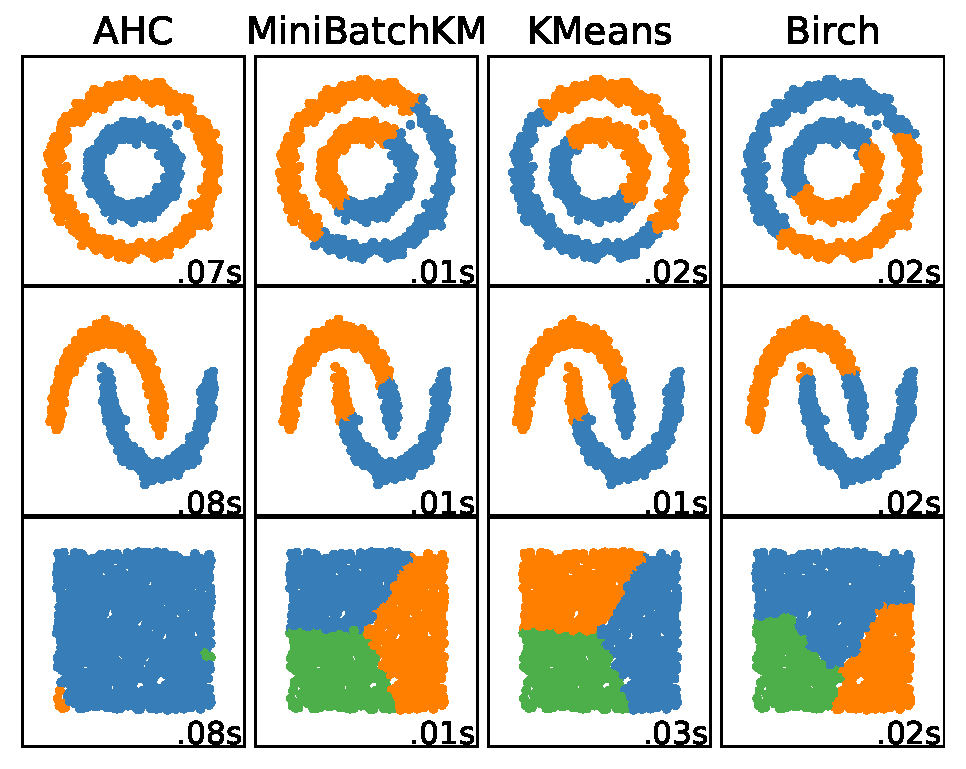
\includegraphics[width=0.8\textwidth]{figures/plots/mlclustering.pdf}
    \caption{The centroids of the AHC cluster in plot a) would both be in the center, placing two CDFs close to each other each representing another circle would not make sense. Mini-batch k-means produces very similar results to k-means with better scaling, only few differences are seen in c). Birch does not produce voronoi clusters, but differences are acceptable, and it scales best for larger data sets.}
    \label{fig:clustering}
\end{figure}
    
We have done extensive tests with k-means clustering, but at first highly underestimated the amount of clusters we need to produce good results. K-means clustering with k-means++ seeding \cite{DBLP:conf/soda/ArthurV07} is considered one of the fastest clustering algorithms with a time complexity of $\bigO(nkdi)$ where $n$ is the number of $d$-dimensional data points, $k$ the number of clusters and $i$ the number of iterations needed to converge. This does work with several million photons and a few dozen clusters, but we found that a typical scene would at least need several thousand CDFs. With a high $n$ and high $k$ scaling quickly becomes a problem again. Quite recent work from \cite{DBLP:conf/kse/HieuM14}, \cite{DBLP:journals/tpds/XuQLMLL14} and \cite{DBLP:conf/www/Sculley10} introduced better scaling to k-means at the cost of slight approximations, which in fact shouldn't really bother us. We especially tried working with the mini-batch k-means algorithm, but once again, scaling was an issue. Our last attempt at a clustering algorithm was Birch \cite{DBLP:conf/sigmod/ZhangRL96} from the sci-kit learn machine learning library \cite{scikit-learn}. Coming closer to our needs, we still were bound by either time or memory, depending on the configuration, and couldn't manage to achieve desirable run times.

We don't bother very much for the exact cluster affinity of single photons, thus a good approximation of spatial subdivision should be enough. This is often not the case for machine learning purposes. Also the dimensionality is often higher. In fact, k-d trees offer exactly this spatial subdivision based on surface area heuristics in 3D (but won't scale for higher dimensions). Even though we found applications of k-d tree as clustering algorithm, it is usually disregarded as not suitable for machine learning applications. With a construction time of $\bigO(n \log n)$ they fit our scalability needs and we can configure how many photons our leafs should maximally have. There are still peculiarities like single photon leafs that we have to handle, we discuss this in section \ref{ch:ev:cdftree}. After the k-d tree is constructed we iterate each leaf, calculate the centroid of each leaf based on the contained photons and construct a CDF to place on that centroid. After all CDFs are constructed we construct a new k-d tree over all CDFs. This k-d tree is then later used for lookups from within the integrator in $\bigO(\log k)$.

Comparing to storing photons we reduced our lookup cost from $\bigO(\log n)$ to $\bigO(\log k)$ and the number of lookups can be significantly lower, as we only care about a smooth interpolation between the CDFs and don't have to worry about missing out on certain light sources. Additionally no hashes have to be computed, instead of a sparse CDF we are constructing an interpolated CDF, which has less overhead attached to it. Nonetheless, we are giving up precision and we are dependent on the quality of our preprocess and interpolation. We discuss interpolating unstructured data points in section \ref{ch:unstructured}.


\section{Interpolation}
\label{ch:interpolation}

In theory, a completely converged picture would always resemble the real light transport in the scene, one would not have to care about variance edges within the scene (as there is none). In practice, we are trying to find good estimators for our importance sampling to reduce processing time. This might work well for certain parts of the scene, but also has a chance to fail for other parts. If the estimator is bad, we sample the important part so rarely (see figure \ref{fig:importancesample}), that this parts might never, or at least extremely slowly, converge, thus sharp variance edges may occur. When the estimator is good for most parts and only bad a few times, this might not be captured by the mean squared error to the reference picture, but human perception is quite sensitive to this variance edges, see figure \ref{fig:varianceEdgeCdfgrid}. As Variance is the margin between estimator and estimated function, variance edges can occur for two reasons, either the estimator does change rapidly, or the scene does change rapidly. Changes of the estimator feel much more unnatural, as we see no apparent reason for those image artifacts, an actual change in the scene (like a hole you are looking through) might not be judged that harshly by a human observer, as the context does change - and with it, the variance\unsure{good?bad?}. With our techniques we always have some spatially precomputed data packets which constitute a discrete representation of our estimators. When estimators are chosen naively this discrete representation shows with unwanted variance edges. We need interpolation to turn this discrete data packets into a continuous and smooth function of estimators. We can't avoid variance in estimator quality, but we try to make it smooth and unnoticeable.

\begin{figure}[htb] 
	\centering
    %\captionsetup[subfigure]{labelformat=empty}

%\begin{tikzpicture}[zoomboxarray, zoomboxarray columns=1, zoomboxarray rows=1]
%    \node [image node] { 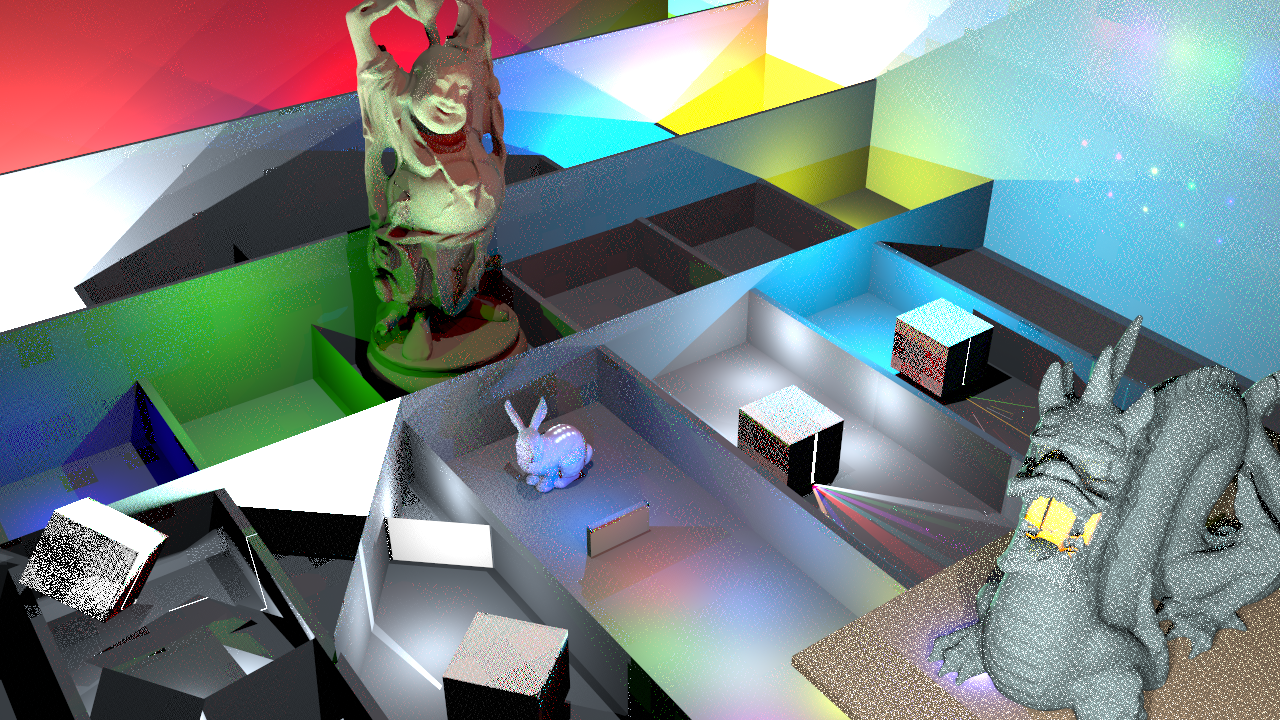
\includegraphics[width=0.5\textwidth]{figures/test2_artifacts.png} };
%    \zoombox[magnification=8,color code=yellow]{0.16,0.72}
%\end{tikzpicture}


\def\infilename{figures/test2_artifacts.png}

\newsavebox{\graph}\savebox{\graph}{\includegraphics[]{\infilename}}
\newlength\gh\setlength\gh{\heightof{\usebox\graph}}
\newlength\gw\setlength\gw{\widthof{\usebox\graph}}

\begin{scaletikzpicturetowidth}{\textwidth}
\begin{tikzpicture}[scale=\tikzscale, >=latex,
  image/.style={anchor=south west,inner sep=0}]
    \ifbool{DEBUG}{
        \node[image] (NI) at (0,0){\phantom{\usebox\graph}};
        \begin{scope}[x={(NI.south east)},y={(NI.north west)}]
            \draw[help lines,xstep=.1,ystep=.1] (0,0) grid (1.001,1.001);
            \foreach \x in {1,...,9} { \node [anchor=north] at (\x/10,0) {\x};}
            \foreach \y in {1,...,9} { \node [anchor=east] at (0,\y/10) {\y};}
        \end{scope}
    };
    \clip (0.4\gw,0.6\gh) rectangle (0.5\gw,0.7\gh);
    \node[image] {\usebox\graph};
    %\draw[|<->|,very thick,red!60] 
    %    (0.5\gw,0.5\gh) -- node[pos=0.5, auto] {$600$} ++(0.2\gw,0\gh);
\end{tikzpicture}
\end{scaletikzpicturetowidth}
    \caption{\textit{Cdfgrid} without interpolation. Even though most of the image is well converged, (b) shows clear variance edges. The CDF construction is dominated by the photons in the darker area, where it works well. The lighting is rapidly changed, the used CDF becomes a bad estimator.} 
    \label{fig:varianceEdgeCdfgrid}
\end{figure}

With our techniques we either collect photons or CDFs, for both methods interpolation is needed, for slightly different reasons. For photons, it does not make sense to only sample one photon, this would imply this shading point would always sample exactly this one light source\footnote{Not exactly, the uniform part of the sparse CDF always contains all light samples with a small probability. Otherwise we would introduce bias.}. We have to collect a bigger set of photons to estimate a good probability distribution of light sources in this area. As this sets gets bigger interpolation gets less important, because for adjacent pixels only a small subset of collected photons change, thus the probabilities and resulting variance changes insignificantly. As we lower the subset to speedup the process, interpolation gets much more important, as individual photons have a higher influence.

With CDFs one might expect considering only the closest CDF might be enough, as a CDF already contains a probability representation for all lights. This might be true for cases when occlusion is not taking into account when the CDFs are calculated. As PBRTs implementation (section \ref{ch:prev:pbrt}) does demonstrate, CDFs are only calculated by distances and angles, due to their spatial correlation adjacent CDFs are similar to each other, thus variance edges are often not noticeable, but still occur, as figure \ref{fig:spatialedge} shows. In that sense, their estimator function is still discrete, but adjacent estimators are by design similar to each other most of the time. This is not true anymore when occlusion is factored in. A single object between two adjacent CDFs could completely change their registered photons. Sampling only the nearest neighbour does result in a very noticeable voronoi diagram, see figure \ref{fig:voronoi}. This can only be solved by interpolation, which generally increases overall variance, but removes those unwanted edges.

The choice which interpolation method can be used highly depends on the fact whether the structure of the data points is known and which structure it has. Interpolating with structured data, especially with a uniform grid, is comparatively fast and easy. We discuss our approach for this case in the following section. For unstructured data, either photons or CDFs, interpolation is harder to achieve without creating artifacts. We considered precomputing a 3D-Delaunay triangulation and applying local interpolation methods, which only makes sense for CDFs, but algorithms like bowyer-watson wouldn't scale well enough for our needs. Additionally, our results indicated, that interpolating within a tetrahedral with only four CDFs, wouldn't mask outlier CDFs well enough. We instead discuss modified global interpolation methods in section \ref{ch:unstructured}. Nonetheless, we acknowledge that there are more interpolation methods or kernels that might be worth to explore.

\subsection{Structured data - Trilinear interpolation}
\label{ch:trilinear}

We apply trilinear interpolation together with the hashed grid in our cdfgrid implementation. Each cell in our hashed grid has 26 neighbours in three dimensions. Based on the shading points location we choose seven neighbours, additionally to the cell itself, to get the eight CDFs $a,b,c,d,e,f,g,h$ at the vertice points with combinations of the coordinates $x_i, x_{i+1}, y_i, y_{i+1}, z_i, z_{i+1}$. Together with the relative coordinates $\alpha, \beta, \gamma$, an interpolation can be calculated with equation~\ref{eq:trilinear} (see also section~\ref{ch:fu:trilinear}).

\begin{align}
    \alpha = \frac{x-x_i}{x_{i+1}-x_i}, \beta = \frac{y-y_i}{y_{i+1}-y_i}, \gamma = \frac{z-z_i}{z_{i+1}-z_i},
\end{align}
\begin{align}\label{eq:trilinear}
    f(\alpha, \beta, \gamma) = a + \alpha\left(b + \beta(e + h\gamma)\right) + \beta(c + f\gamma) + \gamma(d + g\alpha)
\end{align}

As we do not evaluate this equation directly, but rather construct a interpolated CDF to allow for sublinear sampling later on, we have to provide weights for all eight CDFs. We achieve that by transposing equation~\ref{eq:trilinear} as in equation~\ref{eq:trilinearw}, so that the weight per CDF corresponds to the product of relative coordinates in front of it. In fact, the weight is the volume of the opposing cuboid.


\begin{align}\label{eq:trilinearw}
    f(\alpha, \beta, \gamma) &= (1-\alpha)(1-\beta)(1-\gamma)a + (1-\alpha)(1-\beta)\gamma b  \notag \\
    &+ (1-\alpha)\beta(1-\gamma)c  + (1-\alpha)\beta\gamma d \\
    &+ \alpha(1-\beta)(1-\gamma)e + \alpha)(1-\beta)\gamma f \notag \\
    &+ \alpha\beta\gamma g  \notag
\end{align}

\todo{Smooth Step ...}

\subsection{Unstructured data - Shepard interpolation}
\label{ch:unstructured}

Throughout this chapter we argue mostly about interpolating CDFs, most logic can be applied to photons in the same or simpler fashion. The most common method to do global interpolation on unstructured data are Radial Basis Functions (RBF). We considered using RBFs, but found that not only scaling is an issue, but as our function values are N-dimensional CDFs, we were not able to precompute meaningful weights\unsure{maybe just leave that out? Is this correct?}. Also, with RBFs all data points have to be evaluated for a correct result, which is not possible, as we query only some nearest neighbours. Another common approach is to use shepard interpolation to interpolate $\widetilde{f}(x)$ from data points $x_k$ with its corresponding values $f(x_k)$. 

\begin{align}\label{eq:shepard}
\widetilde{f}(x) = \sum_{k}^{N}\frac{w_k(x)}{\sum\nolimits_{j}w_j(x)}f(x_k)
\end{align}

The weight $w_k(x)$ is then only calculated based on distance. A standard approach is to use the inverse distance weight (\ref{eq:inverseDistance}), with parameter $p > 0$ which can be used to smooth the interpolation and $d(x, x_j)$ which is the distance metric (euclidean distance in our case).

\begin{align}\label{eq:inverseDistance}
w_j(x) = \frac{1}{d(x, x_j)^p}
\end{align}

In fact, shepard interpolation is meant to be used as a global interpolation just like RBF. Opposed to RBFs you can use inverse distance weight locally, the function is still interpolated, but looses its continuity, as seen in figure~\ref{fig:lostContinuity}. The reason is, that as you progress through the interpolated function, the outmost nearest neighbour will always snap to another one. With an increasing amount of nearest neighbours the outmost data data point looses significance so the effect becomes less noticeable. But continuity can be restored with the modified shepard method \todo{add cites} where $w_j(x)$ is constructed in such a way, that the outmost nearest neighbour always fade out to zero (equation~\ref{eq:modshep}), therefore the function does not snap when the outmost data value changes.

\begin{align}\label{eq:modshep}
w_j(x) = \left[ \frac{ r - d(x, x_i)}{ rd(x, x_i) } \right]^2
\end{align}

Modified Shepard can be succuessfully used for smooth local interpolation, but inverse distance weighting still has a draw back with our scenario. As $d(x, x_i)$ goes to zero, $w_j(x)$ goes to infinity, this is not only a small implementation problem, but it also creates peaks so that there is always a shading point where a single CDF dominates. This is in fact needed for interpolation and is completely fine for most cases, but we found that in some cases we construct a bad CDF and interpolation with other CDFs won't help at this extreme point, thus leading to variance holes as seen in figure~\ref{fig:varianceHoles}. The only possibility to achieve a smooth appeal is to give up on exact interpolation, but rather approximate the function at the cost of minimally higher overall variance. In fact approximation is what we wanted in the first place, as our underlying CDFs are approximations already, thus strictly interpolating to them is not necessary meaningful in the first place.

A generalization of Shepard interpolation is Kernel Regression (\ref{eq:kernelreg}), where $K(x, x_j)$ is an arbitrary kernel, which opposed to $w_j(x)$ has not to go to infinity when the distance goes to zero, and thus $\widetilde{f}(x)$ approximates instead of interpolates. 

\begin{align}\label{eq:kernelreg}
\widetilde{f}(x) = \sum_{k}^{N}\frac{K(x,x_k)}{\sum\nolimits_{j}K(x, x_j)}f(x_k)
\end{align}

We had good smooth results with a commonly used Gaussian kernel (\ref{eq:gaussiankernel}), but there is a big variety of kernels that can be explored. $p$, again, can be used to define the kernel radius and thus controls the smoothing.

\begin{align}\label{eq:gausskernel}
K(x, x_j) = \mathrm{e}^{-(||x-x_j||/p)^2}
\end{align}

With this approximation approach variance holes are smoothed quite well already. We found that most CDFs were constructed by a similar amount of photons, but there are outliers. That outliers mostly, but not always were assigned just very few photons by the k-d tree clustering. As such one more way to further smooth the image and weaken those outliers is to add a confidence weight $\omega_k$ into Kernel Regression (\ref{eq:ckernelreg}). $\omega_k$ is the number of photons that were used to construct the CDF at $x_k$.

\begin{align}\label{eq:ckernelreg}
\widetilde{f}(x) = \sum_{k}^{N}\frac{K(x,x_k)}{\sum\nolimits_{j}K(x, x_j)}\omega_kf(x_k)
\end{align}


\begin{align}
K(x, x_j)&=\mathrm{e}^{-\left(\frac{||x-x_j||}{p}\right)^2} \\
0.01 &= \mathrm{e}^{-\left(\frac{||x-x_j||}{p}\right)^2} \\
\ln{0.01} &= -\left(\frac{||x-x_j||}{p}\right)^2 \\
\sqrt{-\ln{0.01}} &= \frac{||x-x_j||}{p} \\
p &= \frac{||x-x_j||}{\sqrt{-\ln{0.01}}}
\end{align}


\section{Further Optimizations}



\subsection{Normal culling}






\section{Adaptive Parametrization}

\subsection{Photon Count}

\subsection{Adaptive importance weight}



